\section{Control Charts}
\noindent\rule[\linienAbstand]{\linewidth}{\linienDickeDick}

\subsection{Control Charts versus Hypothesis Testing}
\noindent\rule[\linienAbstand]{\linewidth}{\linienDicke}
\begin{equation}
  \bar{X} \approx \mathcal{N}\left(\mu, \frac{\sigma^{2}}{n}\right)
\end{equation}

% Hypothesis:
% \begin{equation}
%   \begin{split}
%     H_0:& mu = mu_0 (Null-Hypothesis)\\
%     H_1:& mu \neq mu_0 (Alternative-Hypothesis)
%   \end{split}
% \end{equation}


\textbf{Arithmetic mean}
\begin{equation}
  \bar{x} = \frac{1}{n} \sum_{i=1}^n x_i
\end{equation}

Question: is $\left|\bar{x} - \mu_0\right|$ significant
- $\mu_0$ target value\\
- $\bar{x}$ Arithmetic mean of the measurements\\
Given: Level of significantce $\alpha$ = 0.0027

\subsection{Control Charts multiple Measurments per Sample}
\noindent\rule[\linienAbstand]{\linewidth}{\linienDicke}
\begin{figure}
  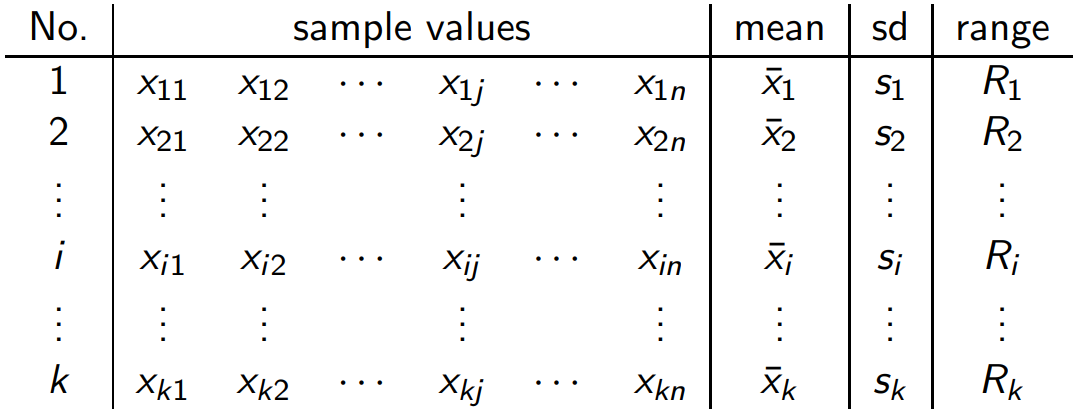
\includegraphics{Pics/2.1.png}
  \caption{Data Set with Mean, Standard Deviation and Range}
  \label{2.1}
\end{figure}

\textbf{Mean values}
\begin{equation}
  \bar{x}_i = \frac{1}{n} \sum_{j=1}^n x_{ij}
\end{equation}

\textbf{Standard deviations}
\begin{equation}
  s_i = \sqrt{\frac{1}{n-1} \sum_{j=1}^n \left(x_{ij} - \bar{x}_i\right)^2}
\end{equation}

\textbf{Ranges}
\begin{equation}
  R_i = max\left \{x_{ij} | j \in \left \{1,...,n\right \} \right \} - min\left \{x_{ij} | j \in \left \{1,...,n\right \} \right \}
\end{equation}
for all $i \in \left \{1,...,k\right \}$

\subsection{R Chart}
\noindent\rule[\linienAbstand]{\linewidth}{\linienDicke}
\textbf{Mean Range}
\begin{equation}
  \bar{R} = \frac{1}{k} \sum^k_{i=1} R_i
\end{equation}

\textbf{Control limits}
\begin{equation}
  \begin{split}
    UCL =& D_4 \bar{R}\\
    LCL =& D_3 \bar{R}
  \end{split}
\end{equation}

\subsection{$\bar{x}$ Chart}
\noindent\rule[\linienAbstand]{\linewidth}{\linienDicke}
\textbf{Mean Range}
\begin{equation}
  \bar{R} = \frac{1}{k} \sum^k_{i=1} R_i
\end{equation}

\textbf{Control limits with sigma}
\begin{equation}
  \begin{split}
    UCL =& \mu + 3 \frac{\sigma}{\sqrt{n}}\\
    LCL =& \mu - 3 \frac{\sigma}{\sqrt{n}}
  \end{split}
\end{equation}
$\mu$: Process mean\\
$\sigma$: Process standard deviation\\
We don't know mu and sigma so we have to estimate them:
\begin{equation}
  E\left(\bar{x}\right) = \mu
\end{equation}
and
\begin{equation}
  Var\left(\bar{x}\right) = \frac{\sigma^2}{n}
\end{equation}
The mean is an unbiased estimator with the standard error
\begin{equation}
  SE\left(\bar{x}\right) = \frac{\sigma}{\sqrt{n}}
\end{equation}
\begin{equation}
  \hat{\sigma} = \frac{\bar{R}}{d_2}
\end{equation}
\begin{equation}
  \bar{\bar{x}} = \frac{1}{k^*} \sum^{k^*}_{i=1} \bar{x_i}
\end{equation}

\textbf{Control limits}
\begin{equation}
  \begin{split}
    UCL =& \bar{\bar{x}} + 3\frac{\bar{R}}{d_2} \frac{1}{\sqrt{n}}\approx \bar{\bar{x}} + A_2 \bar{R}\\
    UCL =& \bar{\bar{x}} - 3\frac{\bar{R}}{d_2} \frac{1}{\sqrt{n}}\approx \bar{\bar{x}} - A_2 \bar{R}
  \end{split}
\end{equation}
